% options:
% thesis=B bachelor's thesis
% thesis=M master's thesis
% czech thesis in Czech language
% slovak thesis in Slovak language
% english thesis in English language
% hidelinks remove colour boxes around hyperlinks

\documentclass[thesis=M,czech]{FITthesis}[2014/05/07]

\usepackage[utf8]{inputenc} % LaTeX source encoded as UTF-8

\usepackage{graphicx} %graphics files inclusion
% \usepackage{amsmath} %advanced maths
% \usepackage{amssymb} %additional math symbols

\usepackage{dirtree} %directory tree visualisation

\usepackage{nameref}

% % list of acronyms
% \usepackage[acronym,nonumberlist,toc,numberedsection=autolabel]{glossaries}
% \iflanguage{czech}{\renewcommand*{\acronymname}{Seznam pou{\v z}it{\' y}ch zkratek}}{}
% \makeglossaries

\newcommand{\tg}{\mathop{\mathrm{tg}}} %cesky tangens
\newcommand{\cotg}{\mathop{\mathrm{cotg}}} %cesky cotangens

% % % % % % % % % % % % % % % % % % % % % % % % % % % % % % 
% ODTUD DAL VSE ZMENTE
% % % % % % % % % % % % % % % % % % % % % % % % % % % % % % 

\department{Katedra softwarového inženýrství}
\title{Adaptibilní systém pro doporučování obsahu}
\authorGN{Jan} %(křestní) jméno (jména) autora
\authorFN{Bouchner} %příjmení autora
\authorWithDegrees{Bc. Jan Bouchner} %jméno autora včetně současných akademických titulů
\supervisor{Ing. Jaroslav Kuchař}
\acknowledgements{Chci upřímně poděkovat všem, kteří mi věnovali čas, když jsem potřeboval pomoc při psaní této diplomové práce, především vedoucímu práce Ing. Jaroslavu Kuchaři za správné směrování, celkový vhled do technologií a cenné komentáře. Děkuji také své rodině a přátelům za bezvýhradnou podporu během celých mých studií.}
\abstractCS{V~několika větách shrňte obsah a přínos této práce v~češtině. Po přečtení abstraktu by se čtenář měl mít čtenář dost informací pro rozhodnutí, zda chce Vaši práci číst.}
\abstractEN{Sem doplňte ekvivalent abstraktu Vaší práce v~angličtině.}
\placeForDeclarationOfAuthenticity{V~Praze}
\declarationOfAuthenticityOption{4} %volba Prohlášení (číslo 1-6)
\keywordsCS{Nahraďte seznamem klíčových slov v češtině oddělených čárkou.}
\keywordsEN{Nahraďte seznamem klíčových slov v angličtině oddělených čárkou.}

\begin{document}

% \newacronym{CVUT}{{\v C}VUT}{{\v C}esk{\' e} vysok{\' e} u{\v c}en{\' i} technick{\' e} v Praze}
% \newacronym{FIT}{FIT}{Fakulta informa{\v c}n{\' i}ch technologi{\' i}}

\begin{introduction}
	%sem napište úvod Vaší práce
	\begin{quote}
		``We are leaving the age of information and entering the age of recommendation''.
	\end{quote}
	Hned na úvod práce jsem si dovolil použít citát z článku \emph{The Long Tail}~\cite{anderson} (česky Dlouhý chvost) bývalého šéfredaktora časopisu Wired Chrise Andersona, který je též autorem stejnojmenné teorie. Ta je založena na tom, že díky internetu lze nabízet širokou škálu produktů, které by dříve mohly jen sotva slavit prodejní úspěchy, neboť poptávka po nich je příliš malá. 
	
	Co je míněno tvrzením \uv{které by dříve mohly jen sotva slavit prodejní úspěchy}?
	
	Myšlenky se lze dopátrat v následující sekci~\nameref{sub:lidinf}, po kterémžto vysvětlení bude vše zasazeno do kontextu zmíněné teorie (podsekce ~\nameref{sub:ltl}) a její souvislosti s potřebou doporučování informací, jež je popsána v sekci~\nameref{sub:recsys}.
	
	Sekce~\nameref{sec:motivation} popisuje vizi systému schopného přizpůsobit se podmínkám a predikovat doporučení na základě předchozích a aktuálních zkušeností.
	
	Popisu nároků na podobný systém, jenž jsem prostřednictvím této práce navrhl a následně implementoval, je věnována sekce~\nameref{sec:objectives}. V sekci jsou též stanoveny cíle, kterých by měl nabývat implementovaný produkt. 
	
	Struktuře práce vzhledem k vytyčeným cílům se věnuje příslušná sekce~\nameref{sec:structure}.
	
\section{Lidstvo a informace}	
	\label{sub:lidinf}
	Význam informací a dat je pro lidstvo odjakživa nezpochybnitelný. Již před nástupem digitálního věku byl jejich objem značný, takže ke spoustě informací, na základě kterých by si byl jednotlivec utvořil vlastní názor, nebylo snadné se dostat.
	
	Lidé se často spoléhali na obecnou oblíbenost daného produktu (ať už se jednalo o zboží, článek, hudebního interpreta a jiné), která byla ale spíše než čímkoliv jiným určována aktuálním společenským trendem nebo informace prostě a jednoduše čerpali ze zkušeností svých několika známých na základě jejich doporučení.

\subsection{Nástup internetu}		
	S masovým rozvojem internetu začalo množství dostupných informací růst obřím tempem (organizace IDC došla v článku \emph{Extracting Value from Chaos}~\cite{digitaluniverse} k závěru, že objem světových dat se každé dva roky zdvojnásobuje). Nové informace jsou produkovány takřka každou sekundu a na jejich setřídění máme mnohem méně času než dříve. Není již v lidských silách udržet si o všem přehled.
	
	Takovým vývojem se přirozeně změnil pohled na data. Cílem není shromáždit co největší objem, neboť při tomto pokusu bychom se zanedlouho dostali do stavu informačního zahlcení. Ceněnou schopností je nyní vytěžit maximální množství užitečných informací a ty využít pro získání nových vědomostí a alespoň přibližně správnou odpověď na otázku potřeb konkrétního jedince.
	
\subsection{Informace a The Long Tail Theory}	
	\label{sub:ltl}
	Vrátím se nyní ještě jednou k teorii Dlouhého chvostu. Pro účely této práce ji nemá význam vysvětlovat dopodrobna, ale je vhodné zmínit alespoň hlavní myšlenku, která vychází z úvah výše.
	
	Nejdůležitějším poznatkem je to, že – z pohledu obchodního – s nárůstem informací dochází k fenoménu snižování prodejů dřívějších hitů (tedy těch několika málo produktů, které se na daném trhu dostanou k masovému publiku, a které určuje především trend) ve prospěch prvků nacházejících se v takzvaném dlouhém chvostu. Uživatel se tak může dostat k informacím, ke kterým by se obyčejným hledáním přes jeden z vyhledávačů třeba nikdy nedostal (pokud by tedy opravdu přesně nevěděl, co hledá).
	
	Bližší představu si lze utvořit při pohledu na obrázek~\ref{fig:longtail}. Na vodorovné ose leží jednotlivé produkty, svislá osa pak znázorňuje objem prodeje (stejně tak se může jednat o popularitu). Žlutá část pod grafem vpravo reprezentuje dlouhý chvost (zhruba 80 procent produktů, po kterých je na trhu poptávka v malých objemech). Zelená část nalevo pak znázorňuje těch několik dominujících produktů (označuje se též jako \emph{hlava}). Tento fenomén lze dobře ilustrovat na příkladu hudebního průmyslu, kde díky obrovským databázím interpretů~\footnote{Jmenujme pár nejznámějších: last.fm, Spotify, Grooveshark, Google Music} již nedochází k selekci a prodeji či poslechu jen těch potenciálně nejúspěšnějších, ale uživatelům se dostává mnohem většího výběru a je jen na nich, kterého si zvolí.
	
\begin{figure}\centering
	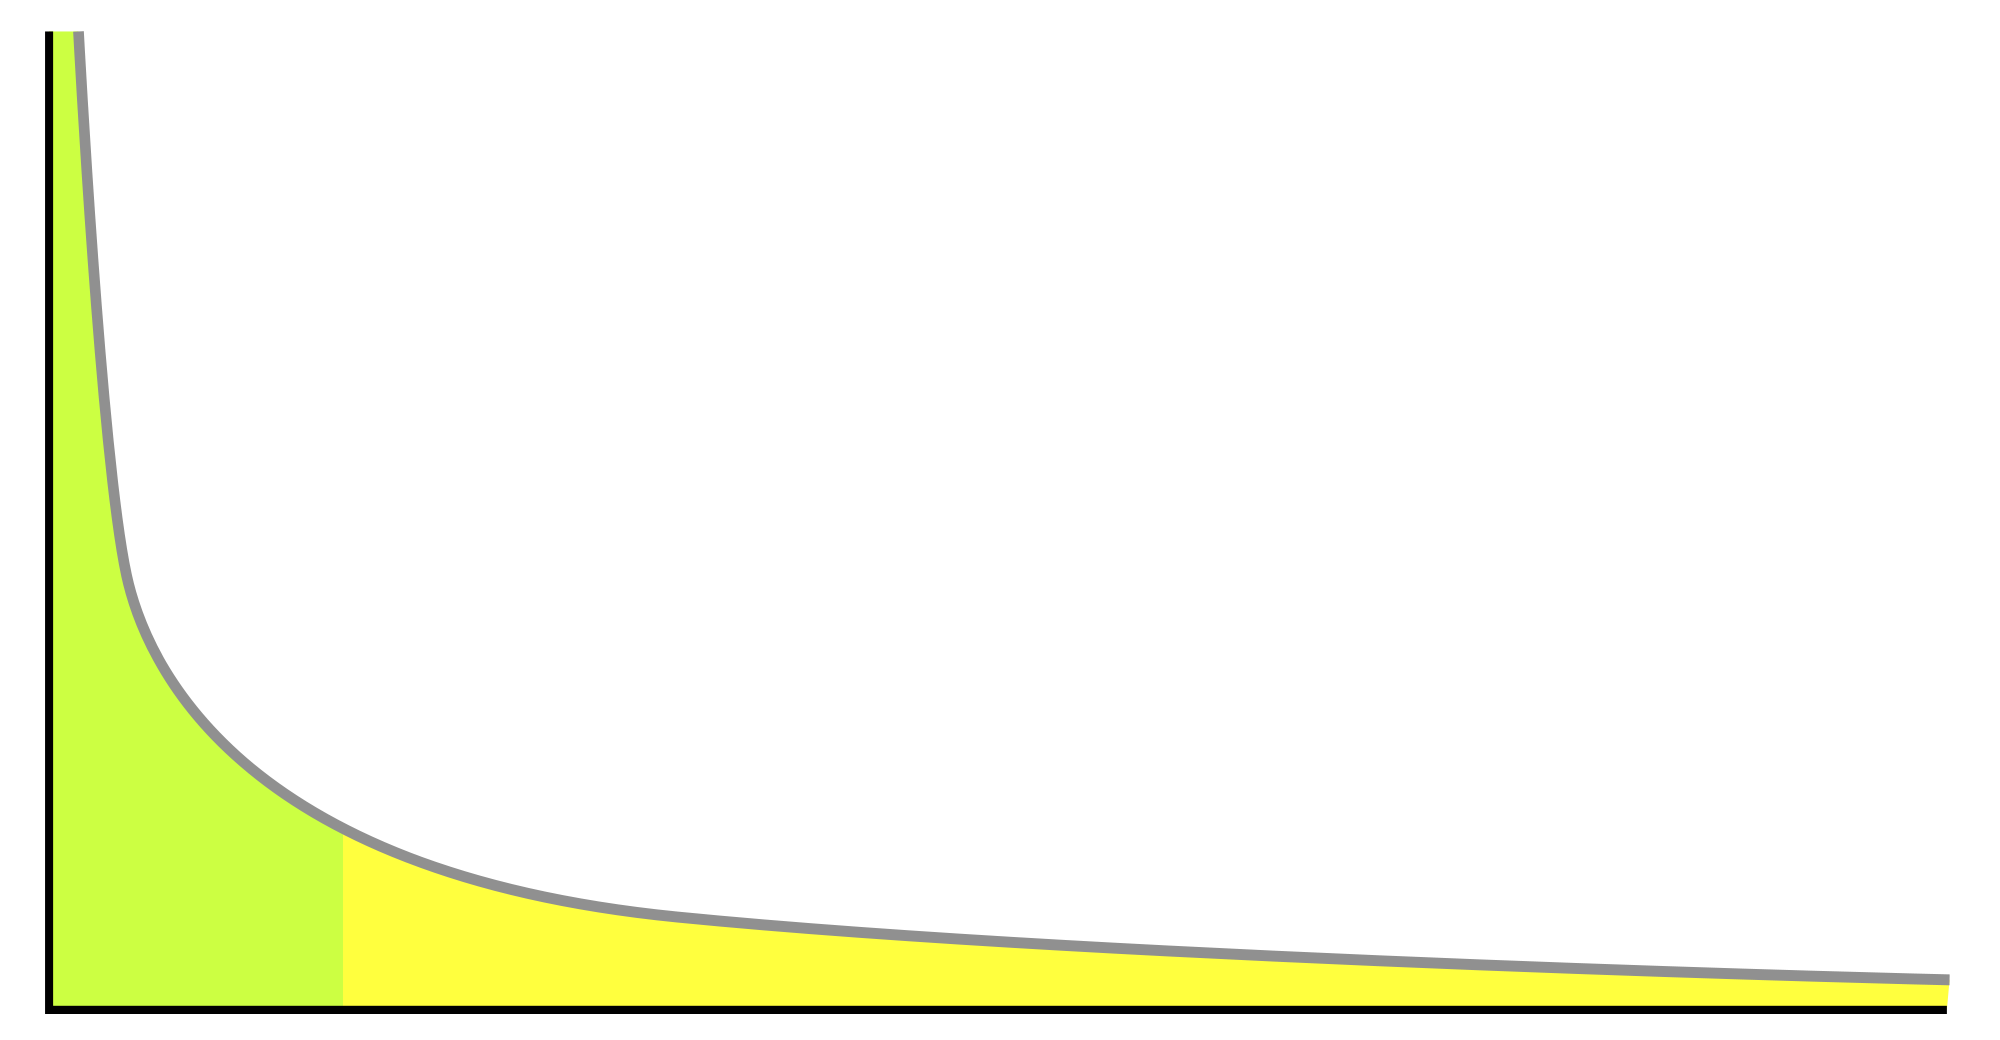
\includegraphics[width=0.8\textwidth]{obr/longtail.png}
 	\caption[Příklad rozdělení zobrazující popularitu hodnocení]{Příklad rozdělení zobrazující popularitu hodnocení. Zdroj: \url{http://en.wikipedia.org/} \cite{wiki:longtail}}\label{fig:longtail}
\end{figure}	

	Všechny výše zmíněné faktory přirozeně zapříčinily rozvoj přístupu zvaného \emph{informační filtrování}, tedy jakési selekce a redukce informací dle volených parametrů. Odtud už byl jen krok k doporučování na míru, které se v posledních několika letech rozmohlo zaváděním tzv. \emph{doporučovacích systémů}.

\section{Doporučovací systémy}
\label{sub:recsys}
 Doporučovací systémy jsou systémy, které mohou být uživateli nápomocné v tom smyslu, že z obrovské množiny informací různými způsoby vyfiltrují relevantní podmnožinu. Například prostým pozorováním toho, jak uživatelé službu využívají (v minulosti zakoupené produkty, seznam všech jimi ohodnocených článků či žebříček preferovaných hudebních interpretů), nebo porovnáváním kontextu uživatele s ostatními lidmi využívajících tu samou službu, lze objevovat pro uživatele nové a jejich vkusu vyhovující položky.
 
\subsubsection{Typy systémů}

Tyto systémy lze dle způsobu práce rozdělit do dvou skupin. 

\begin{description}
	\item[Kolaborativní filtrování.] První skupinou jsou systémy fungující na principu tzv. kolaborativního filtrování. Tento princip má ještě dvě odnože zahrnující doporučování založené na podobnosti uživatelů (user-based) a doporučení založené na podobnosti položek (item-based). Doporučení z této skupiny nejvíce využívají stránky zabývající se prodejem různých produktů a také stránky nabízející novinové články.
	\item[Doporučení založené na obsahu.] Druhou skupinou jsou pak doporučení založená na obsahu. Pro tato doporučení se nejčastěji využívá textové podobnosti. Výhodou je rychlé absorbování nových položek do systému a imunita vůči tzv. \emph{cold start problému}~\footnote{TODO}. Již na malé množině dat lze dostávat poměrně uspokojivá doporučení.
\end{description}
 
 Další informace o doporučovacích systémech a aktuální stav na poli doporučovacích systémů včetně technologického pozadí dokumentuje následující kapitola~\ref{chap:current}. Technické detaily jsou v menší míře k nalezení v sekci~\ref{sec:alg} kapitoly~\ref{chap:impl}.

\section{Motivace} 	
\label{sec:motivation}
		
	Představme si nyní jakéhosi rádce, který dokáže v každém okamžiku rozhodnout, co je za daných okolností nejvhodnější s tím, že to, o čem rádce rozhoduje, je volba algoritmu, kterým by si měl uživatel v danou chvíli nechat doporučit obsah. Pokud by uživatel dbal těchto rad, s největší pravděpodobností by obdržel vhodné doporučení a svou spokojenost by vyjádřil nějakou zpětnou vazbou (tím, že by klikl na doporučené položky nebo by jiným způsobem vyjádřil svůj zájem).
	
	Dokud rádce explicitně nekomunikuje s uživatelem, neprovádí žádné operace a pouze vyčkává na okamžik, kdy bude vyzván k nějaké akci. V okamžiku, kdy je vyzván k tomu, aby uživateli doporučil obsah, je schopen ihned a bez dlouhé analýzy uskutečnit rozhodnutí.
	
	Dokáže též pružně reagovat na situaci, kdy dojde k náhlé změně preferencí nebo vyvstanou jiné nečekané události, které by měli za následek dlouhodobější doporučování nevhodného obsahu.
	
\section{Cíle práce}
\label{sec:objectives}
	Cílem práce je tedy vyvinout rádce popsaného výše, a to ve formě aplikačního software. 

	Nejdůležitějším cílem této práce je tedy návrh a implementace takového adaptibilního systému, jenž by automaticky a vhodně volil a kombinoval metody pro doporučování obsahu. Metodami zde myslí doporučovací algoritmy. Jejich identifikace a výběr vhodné sady je též jednou ze součástí diplomové práce.
	
	Systém bude využívat zpětnou vazbu ohledně kvality doporučení, která principem odměny za dobré doporučení nebo trestu za špatné ovlivní preference při kombinování. Zároveň bude zodpovědný za podporu většího množství uživatelů zasílajících žádosti na systém.
	
	Nezbytnou součástí diplomové práce je též nastudování základních pojmů a pravidel strojového učení a teorie pravděpodobnosti. Zejména kvůli částem zabývajících se zpětnou vazbou a predikcí vhodného algoritmu. 
	
	Vzhledem k fragmentované povaze projektu bude nutné navrhnout obecné rozhraní jak pro doporučovací algoritmy, tak pro adaptibilní systém zahrnující zpětnou vazbu.
	
	K nastudování jsou nutné i technologie pro zpracování většího množství dat a pro rychlou odezvu (ta je potřebná již ze samotné podstaty problému).
	
	Funkčnost navrženého systému by měla být ověřena implementací prototypu a spuštěním na modelové úloze, jež bude simulovat doporučování obsahu pro skupinu více uživatelů.
	
	Tato diplomová práce dokumentuje návrh a vývoj takového systému a s ním spolupracujících komponent. Následuje seznam modulů, které byly pro potřeby práce vyvinuty:

\begin{itemize}
  \item \textbf{adaptibilní systém pro doporučování obsahu}
  \item \textbf{sada základních algoritmů určených k doporučování}
  \item \textbf{rozhraní pro algoritmy a systém pro kombinování}
  \item \textbf{generátor článků, na kterých bylo prováděno základní měření}
\end{itemize}	

\section{Struktura práce}
\label{sec:structure}
	Tato práce je strukturována do 5 různých kapitol a popisuje celý vývojový cyklus systému. Kapitoly jsou řazeny v tom samém pořadí, v jakém probíhaly fáze vývoje.	

\begin{description}
  \item[Kapitola] \nameref{chap:current} popisuje historické pozadí i aktuální trendy používané současnými doporučovacími systémy. Z této rešerše se snaží vyvodit některé závěry, které by mohly být užitečné pro účely některé z dalších kapitol.
  \item[Kapitola] \nameref{chap:analysis} shromažďuje veškeré požadavky kladené na systém, zabývá se návrhem architektury, detailními návrhy serverové i klientské části, rozhraním zastřešujícím komunikaci těchto dvou částí a výběrem základní sady algoritmů, které budou využity k doporučování obsahu. 
  \item[Kapitola] \nameref{chap:adapt} detailně dokumentuje algoritmické a matematické přístupy použité při návrhu adaptibilního systému. 
  \item[Kapitola] \nameref{chap:impl} popisuje vývoj aplikace na základě analýzy a návrhu z předchozích kapitol. 
  \item[Kapitola] \nameref{chap:tests} pak shrnuje poznatky nabyté z experimentů se systémem a hodnotí vyvinutou aplikaci. 
\end{description}
	
\end{introduction}
	
\chapter{Aktuální stav na poli doporučování}	
\label{chap:current}

Kamkoliv v dnešní době na internetu zavítáme, máme velkou šanci, že na některý z doporučovacích systémů narazíme. Mohou mít různá jména:

\begin{itemize}
	\item lidé, které byste mohli znát
	\item uživatelé kupující produkt X kupují též produkt Y
\end{itemize}

Všechny mají ale stejný význam – zaujmout či upozornit na něco nebo někoho konkrétního. Spousta elektronických obchodů, renomovaných aukčních domů, ale též serverů se zábavou na nich doslova staví svá podnikání, neboť správně navržený a fungující doporučovací systém může firmě přinést výrazné zvýšení zisku. 

Sami jejich zákazníci o doporučování stojí. Usnadňují jim navigaci po stránce a existuje vysoká pravděpodobnost, že v závislosti na ní budou přizpůsobovat i své chování. Uživatelská trpělivost ale není neomezená – pokud dostávají špatná doporučení, nenásledují je a ve výsledku odmítají celý systém.

\section{Příklady systémů}
\label{sec:examples}
Na internetu je k nalezení samozřejmě několik desítek – možná stovek – běžících systému, záměrně jsem se proto snažil vybral jen zlomek, který ale pokrývá většinu doporučovaného obsahu (zboží, zábava, text). Níže tedy uvádím jako příklady několik do reálného provozu úspěšně nasazených systémů. 

\subsection{Amazon.com}

\textbf{Amazon.com, Inc.}~\footnote{\url{http://www.amazon.com}} je jedním z nejstarších a největších internetových prodejců. Společnost začínala svůj provoz jako online knihkupectví, ale postupem let zařadila do své prodejní nabídky též hudební a filmové nosiče, software, elektroniku, nábytek a spoustu dalšího zboží.

Novinkou posledních let je vlastní spotřební elektronika v podobě čtečky elektronických knih a tabletů Kindle či poskytování služeb z oblasti cloud computingu.

Firmu lze řadit mezi průkopníky doporučování na internetu. Jako jeden z prvních internetových prodejců totiž začala svým zákazníkům doporučovat výrobky na základě nákupů jiných uživatelů.

Doporučovací systém je založen na několika zdrojích informací:

\begin{itemize}
	\item porovnávání uživatelem prohlížených položek a položek umístěných ve virtuálním nákupním košíku s položkami, které se společně s těmito prohlíženými v minulosti často prodávaly~\footnote{affinity analysis – nacházení spojení mezi odlišnými položkami. Základním příkladem budiž vztah mezi šamponem a kondicionérem. Kupující je většinou používá v ten samý čas~\cite{affinity}. Při nákupu jednoho by mohl mít tedy zájem i o druhý.}.
	\item udržování informací ohledně hodnocení položek uživateli
	\item zaznamenávání historie nákupu (pokud uživatel v minulém měsíci zakoupil tři dětské knížky, znamená to, že má dítě?)
	\item spousta dalších postupů, jako například vyhodnocování demografických informací (dle doručovací adresy), zaznamenávání pohybu po stránce (jaké všechny položky a kolikrát si uživatel prohlédl, než umístil jednu konkrétní do nákupního košíku) nebo sledování prokliků~\footnote{Jako proklik se označuje takové kliknutí na odkaz, které uživatele dovede na cílovou stránku~\cite{proklik}.} z cílených marketingových e-mailů s odkazy na zboží~\cite{amazonrec}.
\end{itemize}

Společnost nazývá svou hlavní doporučovací strategii jako \emph{item-to-item kolaborativní filtrování} a používá ji pro přizpůsobení prohlížení webu svým stálým zákazníkům. V tom smyslu, že fanoušek moderních technologií může při své návštěvě stránek nalézt odkazy na technologické novinky všeho druhu, zatímco mladá matka bude mít na těch samých stránkách v nabídce ve větším zastoupení dětské zboží.
 
Výše jsou popsány pouze základní principy. Doporučovací systém společnosti je samozřejmě velmi komplexní a detailní algoritmus je udržován jako obchodní tajemství. K nahlédnutí jsou ale patenty, např. \emph{Personalized recommendations of items represented within a database}~\cite{jacobi2006personalized} nebo \emph{Collaborative recommendations using item-to-item similarity mappings}~\cite{linden2001collaborative}.

\subsection{Netflix}

\textbf{Netflix, Inc.}~\footnote{\url{https://www.netflix.com}} je společnost, která začínala nabízet své služby jako internetová videopůjčovna. Během posledních pár let (strategicky významný byl rok 2007, kdy byla nabídka rozšířena o filmy streamované prostřednictvím internetu~\cite{netflix2007}) se rozrostla v obrovskou mediální společnost nabízející obsah v podobě filmů a seriálů pro většinu v dnešní době používaných platforem jako PC, Mac, PlayStation3, Wii, Xbox a také mobilní telefony a tablety. 

Vzhledem k tomu, že firma staví své podnikání na tom, že přicházející uživatelé platí za konzumaci zábavy (dle~\cite{netflixrec} pochází 2/3 zapůjčených filmů z předchozího doporučení), je v jejím vlastním zájmu, aby těmto uživatelům sledujícím filmy a seriály nabízela automaticky další obsahově či žánrově podobné, zkrátka takové, jenž budou co možná nejvíce lahodit jejich vkusu. Úspěšné podnikání společnosti je tak přímo závislé na tom, jak kvalitním doporučovacím systém společnost disponuje. 

\subsubsection{Netflix Prize}

Za účelem zkvalitňování doporučování filmů byl vyvinut vlastní systém s názvem \emph{Cinematch}. Potřeba neustálého zlepšování a zpřesňování doporučení vyústila ale v to, že společnost začátkem října 2006 vypsala soutěž známou jako \emph{Netflix Prize}. Jednalo se o pokus ještě více pokročit na poli doporučování filmů a pro tým, který by dokázal zlepšit dosavadní výsledky systému Cinematch alespoň o 10 procent, byla vypsána odměna ve výši 1 000 000 dolarů.

K tomuto účelu společnost uvolnila testovací data obsahující ID uživatele, ID filmu, hodnocení na intervalu <1,5> a datum uskutečnění hodnocení. Testovací data obsahovala 100 480 507 hodnocení pro 17 770 filmů od 480 189 uživatelů. Uvolněna byla ještě další testovací data obsahující stejné informace, jen byla vynechána uživatelská hodnocení. Cílem úkolu pak bylo předpovědět tato chybějící hodnocení opět na intervalu <1,5>.

Cena byla udělena až v roce 2009 (do té doby docházelo k průběžnému zlepšování, ale nebylo dosaženo stanoveného zlepšení o 10 procent) týmu \emph{BellKor's Pragmatic Chaos} (který vznikl spojením tří do té doby samostatných týmů). Vítězný tým použil k dosažení cíle technik strojového učení, aby při tom zjistil několik zásadních poznatků. Například to, že každé hodnocení filmu je silně subjektivní záležitostí, kterou je dopředu obtížné předpovědět. Ukázalo se také, že velmi záleží na tom, zda uživatel hodnotí právě dosledovaný film nebo film, který zhlédl již před delší dobou. Velkou roli též hraje nálada během dne a další faktory~\cite{bellkor}.

Výsledný algoritmus je navíc směsicí zhruba stovky menších algoritmů, takže by se dalo s trochou nadsázky prohlásit, že jednou z hlavních taktik je použít tolik doporučovacích algoritmů, kolik je jen možné. 

\subsection{Zite}

\textbf{Zite.com}~\footnote{\url{http://zite.com}} je moderní aplikace pro chytré mobilní telefony a tablety.

Mike Klass, CTO společnosti v jednom z článků~\cite{ziteflip} prozradil, že vizí bylo vyvinout sofistikovaný, na technikách strojového učení postavený systém, jehož účelem nebude pouhé filtrování příchozích novinek vedoucí k úspoře času uživatele. Cílem tohoto systému bylo přizpůsobit se svému uživateli studiem vzorců chování (pozoruje zájmy a návyky při čtení článků) natolik, aby mu dokázal doporučit přesně to, co v danou chvíli hledá, ale kvůli různým okolnostem (například obsah produkovaný neznámým bloggerem) by na to nikdy neměl šanci narazit.

Zite nasazené v systému uživatele je tedy stejně tak unikátní jako jeho uživatel. Sleduje, jaké článků si vybírá ke čtení, jak dlouhé tyto články jsou a jak dlouho stráví uživatel jejich čtením. Systém tedy každý den vyhodnocuje miliony nových článků, přičemž se zaměřuje na typ, klíčové atributy i na to, jakým způsobem je článek sdílen skrze web. Následně využije tyto informace ke spárování vybraných článků s osobním vkusem uživatele a tyto články mu doručí do aplikace. 

Tak jako Netflix a Amazon doporučují filmy a produkty, které by na základě podobnosti mohli uživatele zajímat, stejně tak i Zite provádí na pozadí porovnání mezi čtenáři – jak v rámci aplikace, tak obecně na webu.

\subsubsection{Zite \& CNN \& Flipboard}
V srpnu 2011 o technologii vyjádřila zájem společnost CNN~\cite{zitecnn} a Zite přešlo pod ni. Poslední novinky ze začátku března 2014 ale naznačují~\cite{ziteflip}, že Zite opouští CNN a rozhodlo se spojit síly s aplikací Flipboard~\footnote{https://flipboard.com} vývojářské společnosti Flipboard, Inc., jejíž funkcionalitou je agregování obsahu ze sociálních sítí a jiných stránek a následné nabízení ke čtení v magazínovém formátu umožňujícím jednoduchým způsobem listovat napříč vzájemně souvisejícími tématy.

Společným cílem je vystavět nejlepší systém pro personalizované čtení novinek. 

\subsection{Mendeley}	

\textbf{Mendeley}~\footnote{\url{http://www.mendeley.com}} je systém určený k doporučování vědeckých článků využívající jako svou výpočetní vrstvu technologii Apache Mahout~\footnote{https://mahout.apache.org}. Cílem systému je spojovat dohromady výzkumníky a jejich data. Svým uživatelům tak pomáhá v organizaci výzkumu, umožňuje jim nalézt potenciální spolupráci s dalšími uživateli aplikace a napomáhá též k objevům nových podnětů pro vlastní práci. Uživateli této aplikace jsou přední světové university jako University of Cambridge, Stanford University, MIT či University of Michigan. Data pro aplikaci pocházejí z vlastních importů svými uživateli i z externích importů skrze různé katalogy prací. 

Projekt samotný se v jedné ze svých prezentací~\cite{mendeleylastfm} přirovnává k největší hudební databázi na internetu – last.fm~\footnote{http://www.last.fm}. Ta funguje na tom principu, že potenciální uživatel si nainstaluje na svůj počítač desktopovou aplikaci, následně s instalovanou aplikací začne poslouchat hudbu a tím je zahájeno automatické odesílání informace o skladbě (interpret, žánr apod.) na server last.fm. Podle těchto odeslaných dat jsou uživateli v budoucnu doporučovány další skladby. 

Mendeley tuto analogii vysvětluje tím, že hudební knihovny jsou v jeho případě výzkumné knihovny, roli interpretů zde zastávají jednotliví výzkumníci, hudební skladby jsou pak jimi publikované články a jednotlivé hudební žánry reprezentují vědecké disciplíny.  

Doporučení jsou zde generována dvojím způsobem. 

\begin{description}
	\item[Kolaborativní filtrování] Používá se pro personalizované doporučení. Podporována je jak user-based, tak i item-based varianta doporučení.
	\item[Filtrování založené na obsahu] Používá se k nalezení souvisejícího výzkumu, například nalezení článku ze stejné výzkumné kategorie nebo článku s podobným názvem. 
\end{description}

Uživatelé mohou svůj zájem či nezájem o každou z doporučených položek vyjádřit zpětnou vazbou, která je dvojího typu:

\begin{description}
	\item[Accept] Vyjadřuje, že uživatel s daným doporučením souhlasí nebo pro něj vylo nějakým způsobem užitečné.
	\item[Remove] Vyjadřuje nevhodné doporučení. Uživatel touto volbou dává najevo, že podobné doporučení by raději již příště nedostal.
\end{description}

\subsection{Google News}	

Vlastní platformu pro doporučování obsahu má jako součást svého vývoje též společnost \textbf{Google, Inc.}~\footnote{\url{http://www.google.com/about/company}}. Její výzkumníci se ve své práci~\cite{googlenews} zabývali vývojem prediktivního systému pro personalizované doporučování zpráv na webu Google News~\footnote{\url{http://news.google.com}}. Přihlášeným uživatelům, kteří mají v prohlížeči explicitně povolen záznam historie, jsou generována doporučení založená na zájmu těchto uživatelů vycházejících z profilů sestavených pozorováním chování na stránce.  

K porozumění, jak se mění zájem uživatelů o zprávy v čase, napomohla výzkumníkům analýza logů (záznamy chování anonymních uživatelů na stránce). Na základě této analýzy byl vyvinut Bayesovský framework pro předvídání zájmu uživatelů o novinky.

Kombinací mechanismu pro filtrování informací, který vzešel z předpovězených uživatelských profilů a již existujícího mechanismu využívajícího principů kolaborativního filtrování vznikl systém pro generování personalizovaných zpráv. Tato kombinace byla nasazena do živého provozu a následné experimenty prokázaly, že kombinováním metod došlo ke zlepšení kvality doporučování, což vedlo k častějším návratům na stránky.

\subsection{Výzkum}

Také současný výzkum v oblasti doporučovacích systémů, zdá se, nezahálí. Zde je výčet několika akcí, jejichž náplní či součástí je problematika doporučování a doporučovacích systémů.

\begin{itemize}
  \item \textbf{ACM RecSys conference.}~\footnote{\url{http://recsys.acm.org}} Tato konference je předním mezinárodním fórem pro prezentaci nových výsledků výzkumu a postupů na poli doporučovacích systémů. RecSys sdružuje hlavní mezinárodní výzkumné skupiny a též mnoho předních světových společností na trhu e-commerce. Nabízí také doprovodný program v podobě zvaných přednášek, konzultace týkající se problematiky RecSys a sympózium studentů doktorských programů. 
  
  Zajímavé prezentace jsou volně dostupné na internetu, dá se tedy načerpat spousta inspirace do vlastního výzkumu. Mně osobně velmi zaujala prezentace~\footnote{\url{http://www.slideshare.net/d0nut/open-recommendation-platform}} z posledního ročníku konference (Hong Kong, 2013), se kterou vystoupil jeden z klíčových řečníků Torben Brodt. V prezentaci popisuje tzv. \emph{Open Recommendation Platform}, která je založena na výběru vždy toho nejlepšího algoritmu pro doporučení v závislosti na daném kontextu. 
  
  \item \textbf{ICWSM: Weblog and Social Media.}~\footnote{\url{http://www.icwsm.org/2014}} The International AAAI Conference on Weblogs and Social Media je mezinárodní konference, na které se střetávají výzkumní pracovníci z oblasti počítačových a společenských věd. Konference je pořádaná za účelem sdílení znalostí, diskutování o nápadech a výměny informací. Probíranými body jsou psychologické a sociální teorie, výpočetní algoritmy pro analýzu sociálních médií a jedním z mnoha témat jsou též doporučovací systémy.
  \item \textbf{ICML: Machine  Learning.}~\footnote{http://icml.cc/2014} The International Conference on Machine Learning je konference s bohatou historií. Její první ročník proběhl již v roce 1980 v Pittsburghu. Jedná se o přední mezinárodní konferenci zabývající se strojovým učením. 
\end{itemize}

O tématu se též píše spousta článků a každým rokem vzniká několik disertačních prací. Dle dostupných informací z ACM RecSys Wiki~\footnote{\url{http://www.recsyswiki.com/wiki/List_of_recommender_system_dissertations}} jich jen za poslední 4 roky bylo přes 50. 

\section{Shrnutí poznatků}

Z výše uvedených příkladů~\ref{sec:examples} lze vypozorovat určité společné vlastnosti a zformulovat několik závěrů:

\begin{itemize}
	\item o uživateli je vedena spousta záznamů, například historie jeho chování na stránkách
	\item velký důraz je kladen na zpětnou vazbu (vyjádření zájmu uživatele o obsah stránky)
	\item stále se využívá osvědčených přístupů kolaborativního filtrování a filtrování na základě obsahu
	\item síla není v použití jednoho konkrétního algoritmu, ale v kombinaci více metod a přístupů dohromady
	\item většina výpočtů běží na pozadí v tom samém čase, co uživatel tráví prohlížením stránek, a je schopna se přizpůsobit okolnostem
	\item problematika má silnou závislost na strojovém učení a teorii pravděpodobnosti
\end{itemize}

Existujících řešení je tedy celá řada. Každé z těchto řešení je ale využíváno ke svému vlastnímu účelu a není vzájemně přenositelné. Navíc se zdá, že době, kdy obchodníkům stačilo na svůj elektronický obchod nasadit jednoduchý algoritmus kolaborativního filtrování, již odzvonilo a budoucnost patří systémům schopným přizpůsobit vývoj doporučování dle nějaké predikce, a to navíc v reálném čase. 

\chapter{Analýza a návrh řešení}
\label{chap:analysis}

Zatímco v předchozí kapitole jsem se zabýval popisem existujících řešení a zkoumal, jaké možnosti nabízejí současné doporučovací systémy, tato kapitola je celá věnována analýze požadovaného chování mnou vyvíjeného systému.

Nejprve se budu zabývat požadavky na systém, které vyplynuly z úvodních konzultací s vedoucím práce a vlastním zkoumáním problému. Se znalostí těchto požadavků bude možné provést hrubý návrh architektury systému včetně technického řešení součástí, kterými bude systém disponovat.

Prostřednictvím výstupů získaných v této kapitole budu schopen provést implementaci systému.

\section{Požadavky}

Za účelem vyšší přehlednosti jsem se nejprve rozhodl související požadavky strukturovat do zastřešujících skupin trojího typu (globální požadavky, rozhraní a systém). Nakonec se ale ukázalo, že mezi skupinami \emph{rozhraní} a \emph{systém} existuje velmi tenká hranice (z hlediska požadovaného chování, nikoliv implementačního), proto byly skupiny redukovány na dvě.

\subsection{Globální požadavky na systém}

\begin{itemize}
	\item Systém bude mít možnost uložit v pravidelných intervalech svůj aktuální stav pro potřeby obnovení v případě pádu.
	\item Bude existovat možnost zobrazení dosavadního průběhu doporučování systémem v čase.
	\item Systém bude veškerou komunikaci vyhodnocovat v reálném čase (live read, live write).
	\item Systém bude na každou žádost vracet příslušnou odpověď (i chybovou).	
	\item Systém poklade důraz na zpětnou vazbu, podle které bude přizpůsobovat své chování.
	\item Zpětná vazba bude realizována na principu odměny za dobré doporučení (přičítání) a trestu za špatné (odečítání).
	\item Systém se bude automaticky přizpůsobovat vývoji v čase tím, že bude normalizovat své hodnoty (aby nedošlo k přetečení datových typů).
\end{itemize}

\subsection{Systém \& Rozhraní}

\begin{itemize}
	\item Systém bude umožňovat vytvářet skrze své rozhraní kolekce s algoritmy určených pro následnou predikci. 
	\item Uživatel bude mít možnost zaslat systému svou žádost o radu a obdržet informaci o tom, který algoritmus pro doporučení obsahu by měl v danou chvíli zvolit.
	\item Uživatel bude mít možnost zaslat systému informaci o tom, jaký algoritmus pro doporučení se rozhodne vybrat.
	\item Uživatel bude mít možnost zažádat o doporučení obsahu pomocí algoritmu, který mu byl navržen systémem.
	\item Uživatel bude mít možnost zaslat systému zpětnou vazbu pro zvolené doporučení.
	\item Aplikace bude umožňovat skrze své rozhraní zpracovávat informace o tom, že jeden uživatel dělá něco s jedním dokumentem (zpracování zpětné vazby).
	\item Aplikace bude umožňovat skrze své rozhraní mazat pro doporučování již neaktuální informace. 
\end{itemize}

Dle disciplín softwarového inženýrství je výčet uvedený výše nazýván jako \emph{funkční požadavky}.

Lze definovat i tzv. \emph{nefunkční požadavky} specifikující vlastnosti a omezující podmínky kladené na systém:

\begin{itemize}
	\item Systém bude postaven na platformě Java.
	\item Rozhraní systému bude navrženo a implementováno v podobě služeb REST (vychází ze zadání)
	\item Systém bude postaven tak, aby se dal snadno parametrizovat. 
	\item Systém bude připraven na to, že jej bude využívat více uživatelů současně.
	\item Systém poběží jako samostatná aplikace. Ostatní s ní budou komunikovat zvenčí.
	\item Systému bude pro snadné nasazení a otestování vytvořen cookbook nástrojem Chef a bude jej možno nasadit nástrojem Vagrant.
\end{itemize}

\section{Adaptibilní systém}

Pro implementaci systému splňujícího požadavky vzešlé z analýzy výše je třeba důkladně zvážit, jaké všechny komponenty bude obsahovat a případně jaké algoritmické postupy bude nutné použít. Na základě zkoumání existujících implementací v kapitole~\ref{chap:current} mě velmi zaujal projekt \emph{Open recommendation Platorm} (zkr. ORP) společnosti plista~\footnote{\url{https://www.plista.com}} prezentovaný na posledním ročníku konference ACM RecSys 2013 v Hong Kongu. 

Motivací ORP bylo získat lepší výsledky kombinací více doporučovacích metod společně se zapojením kontextu uživatele, neboli informacemi čerpanými převážně z HTTP hlaviček. Těmi informacemi mohou být:

\begin{itemize}
	\item IP adresa, která může prozradit geologickou lokaci uživatele
	\item denní doba, kdy je ke stránce přistupováno
	\item user agent informující o zařízení, ze kterého bylo k obsahu přistoupeno (mobilní telefon, PC)
	\item referer pro zjištění způsobu přístupu (přístup z vyhledávání nebo přímý přístup) 
\end{itemize}

Abstraktní pohled na ORP znázorňuje obrázek~\ref{fig:plista}. Na něm je systém zachycen jako \emph{Ensemble}, který je dle uživatelských preferencí schopen vybírat z kolekce doporučovacích algoritmů ten nejvhodnější, který použije pro publikování obsahu. Konzumenti doporučeného obsahu (\emph{Visitors}) pak zasílají systému zpětnou vazbu, kterou systém použije k přepočítání preferencí, čímž ovlivní výběr budoucího algoritmu.

\begin{figure}\centering
	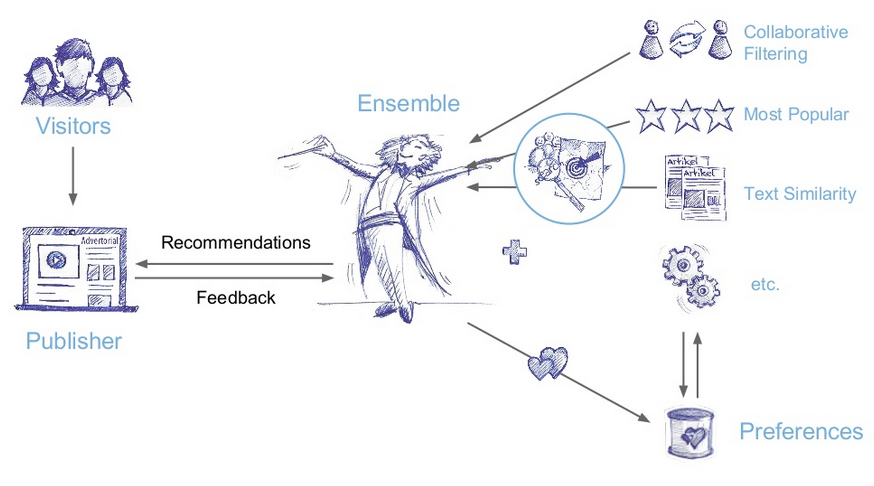
\includegraphics[width=1.0\textwidth]{obr/plistaEnsemble.png}
 	\caption[Abstraktní pohled na systém společnosti plista]{Abstraktní pohled na systém společnosti plista. Zdroj: \cite{slideshare:plista}}\label{fig:plista}
\end{figure}	

V prezentaci bylo zmíněno několik dobře míněných rad ohledně toho, co by měl systém podobného typu umět. Zmíněna je potřeba rychlého webového serveru, na kterém bude aplikace běžet, dále nutnost rychlého síťového protokolu a rychlé fronty zpráv. Padla zde též nutnost rychlého úložiště dat. K dosažení funkcionality pro výběr nejlepšího algoritmu za daných podmínek společnost používá tzv. \emph{multi-armed bayesian bandit}, což byla i jedna z doporučovaných strategií, které mi na úvodní schůzce doporučil vedoucí práce.

Se spoustou rad jsem se ztotožnil a vyhodnotil, že s jejich pomocí bych mohl být schopen uspokojit velkou část požadavků na systém stanovených výše.

Strategie \emph{multi-armed bayesian bandit} je pro mou práci natolik významná, že jsem jí věnoval samostatnou kapitolu~\ref{chap:ensemble}.

\section{Architektura systému}

\subsection{Server}

\subsection{Klient}

\subsection{Komunikace}

že to bude komunikovat skrz to rozhraní co je popsaný tam a tam. 
	
\section{Sada algoritmů}
Identifikujte sadu základních algoritmů určených pro kombinování. Ty implementujte nebo použijte existující implementace.	

\subsection{Algoritmus náhodného výběru}

\subsection{Algoritmus výběru dle nejnovějších položek}

\subsection{Algoritmus výběru nejlépe hodnocených položek}

\subsection{Algoritmus výběru dle podobnosti obsahu}

\subsection{Algoritmus kolaborativního filtrování}

\section{Rozhraní}

normálka návrh endpointů a tak

Z prováděné analýzy vyplývají požadavky na rozhraní tak, že jej můžeme rozdělit do tří skupin dle úkolu:

\subsection{Rozhraní pro adaptibilní systém}

\begin{itemize}
	\item vytvořit kolekci banditů
	\item 	provést dotaz na kolekci banditů (na nejlepší algoritmus nebo na seřazené pořadí)
	\item 	zaslat informaci o tom, že bandita byl vybrán pro doporučení
	\item zaslat systému feedback s tím, jak jsem byl s volbou spokojený		
\end{itemize}

\subsection{Rozhraní pro sadu základních algoritmů}

\begin{itemize}
	\item zaslání žádosti o doporučení obsahu konkrétním algoritmem
\end{itemize}

\subsection{Rozhraní pro úložiště dat}

\begin{itemize}
\item zaslání informace o tom, že 1 uživatel dělá něco s jedním článkem
	\item smazání/zneviditelnění článku z výsledků hledání
\end{itemize}

\section{Formát vyměňovaných zpráv}

Popsat ten JSON a tak
			
\chapter{Adaptibilní systém}
\label{chap:adapt}
Navrhněte, implementujte a otestujte systém, který bude dynamicky kombinovat algoritmy a optimalizovat celkovou kvalitu algoritmů.
\label{chap:ensemble}

\section{Strojové učení}

Vzhledem k povaze řešeného problému je nutné zaměřit se na metody tzv. \emph{strojového učení}. 
Jedná se o vědeckou disciplínu (jednu z větví oboru umělé inteligence), která se zabývá tím, jak se má počítač přizpůsobit určité situaci, aniž by byl pro danou situaci explicitně naprogramován. Metody strojového učení, které hledají generalizaci libovolných dat nebo slouží pro adaptaci existujícího systému na změny okolí, se používají ve všech oblastech informačních věd od analýzy snímků, analýzy DNA a textu, až po simulace chování člověka. 

Typickým příkladem je vytvořit z dostupných dat model, který dokáže:

\begin{itemize}
  \item predikovat cenu akcií za 6 měsíců z aktuální výkonnosti společnosti a ekonomických dat
  \item rozpoznat spam od regulérního e-mailu
  \item u pacienta hospitalizovaného s infarktem predikovat riziko dalšího infarktu
  \item napomoci společnostem zabývajících se internetovou reklamou v rozhodování se, kterou reklamní strategii použít k maximalizaci zisků
  Používá to ale třeba Google analytics! při správě online experimentů
\url{https://support.google.com/analytics/answer/2844870?hl=cs&ref_topic=2844866}
\end{itemize}

Algoritmy strojového učení mohou být děleny do taxonomie (nadtříd a podtříd) založené na požadovaném výsledku algoritmu nebo typu vstupu, který je k dispozici během trénování stroje. Algoritmů je celá řada, bude tedy vhodné zmínit zde alespoň ty nejtypičtější. 

\begin{description}
  \item[Supervised learning]~\footnote{učení s učitelem} TODO
  \item[Unsupervised learning]~\footnote{učení bez učitele} TODO
  \item[Reinforcement learning]~\footnote{zpětnovazební učení nebo též učení posilováním} TODO
\end{description}

TODO zmínit, že pro naše potřeby je nejvhodnější reinforcement learning.

\url{http://cs.wikipedia.org/wiki/Strojov%C3%A9_u%C4%8Den%C3%AD}
\url{http://cs.wikipedia.org/wiki/Zp%C4%9Btnovazebn%C3%AD_u%C4%8Den%C3%AD}
\url{http://en.wikipedia.org/wiki/Machine_learning}
\url{http://cs.wikipedia.org/wiki/U%C4%8Den%C3%AD_s_u%C4%8Ditelem}
\url{http://en.wikipedia.org/wiki/List_of_machine_learning_algorithms#Supervised_learning}
\url{http://en.wikipedia.org/wiki/Reinforcement_learning}
\url{http://tdunning.blogspot.cz/2012/10/references-for-on-line-algorithms.html}
\url{http://tdunning.blogspot.cz/search?q=bandit}
\url{http://camdp.com/blogs/multi-armed-bandits}
\url{http://www.recsyswiki.com/wiki/Ensemble}

Algoritmus začne ve stavu nevědomí (ignorant state), kdy neví nic o daných okolnostech a začíná nabývat vědomosti tím, že testuje systém. Tím, jak vstřebává data a vyhodnocuje výsledky, učí se, jaké chování je nejlepší.

Z psychologického hlediska se jedná o následující úvahu: Jakým způsobem dokáže trest a odměna ovlivňovat naše budoucí chování? Na základě čeho se (nejen) lidstvo učí novým věcem?

\subsection{Online učení}

Navrhovaná strategie je též nazývána jako \emph{online učení}. Nutno zmínit, že slovem online zde není míněno něco ve smyslu internetu, ale ve smyslu neustále se vyvíjející aktualizace dat. Učící algoritmus v každém kole vykoná nějakou akci, přijme zpětnou vazbu a připíše si daný zisk či ztrátu.

Z matematického hlediska má online učení propojení na klasické online algoritmy, teorii (opakovaných) her a teorii pravděpodobnosti. Díky těmto znalostem tak můžeme navrhovat pravděpodobností dynamické systémy, kterými lze modelovat složitá průmyslová zařízení nebo třeba výherní automat známý jako mnohoruký bandita (Multi-Armed Bandit).

\section{Multi-armed Bandit algoritmus}
The Multi-Armed Bandit Problem je jedním z klasických problémů online učení. Tato herní strategie je podobná tradičnímu hernímu automatu, který představuje one-armed strategii, ale mnohoruká varianta má více herních pák~\emph{V každém kole si lze pro hru vybírat mezi N automaty}. 

\subsection{Princip algoritmu}
Strategii si lze představit tak, že stojíme před N výherními automaty (též nazývány jako bandité) a v každém kole máme možnost vybrat si jeden z nich, na kterém budeme hrát. Pravděpodobnosti výher u jednotlivých automatů jsou pro nás neznámé. 

Formálně lze strategii popsat jako skupinu výnosových (reward) distribučních funkcí B = {R1, …, RK}, kde K je počet banditů. Každý bandita má tedy přiřazenu jednu distribuční funkci, jež vyjadřuje pravděpodobnost úspěchu. 

Zpočátku nemá hráč žádnou informaci o průběhu hry ani o rozložení pravděpodobnosti úspěchu napříč bandity. Tím, že v každém kole vybíráme vždy jen jednoho banditu, se snažíme navrhnout strategii pro maximalizaci celkové výhry.

Samozřejmě, že kdybychom znali banditu s největší pravděpodobností výhry, potom bychom jej vždy vybírali, čímž bychom maximalizovali výhry. Naším úkolem bude tedy nalézt nejlepšího banditu a to co nejrychleji, jak je to jen možné.

K návrhu strategie nám pomáhá to, že jednotlivé bandity nejdříve testujeme, abychom získali nutné znalosti. Poté už se lze zaměřovat na páky, které nám poskytují největší zužitkované znalosti. 

Úkol trochu komplikuje stochastická povaha banditů. Suboptimální bandita může vracet spoustu výher, což by nás mohlo přimět uvěřit, že právě tento bandita je velice štědrý. Podobně ale naopak nejlepší bandita může vracet spoustu proher. Měli bychom tedy pořád zkoušet i lůzry, nebo se na ně vykašlat?

Co je dalším problémem, tak pokud najdeme banditu, který vrací “docela dobré” výsledky, měli bychom toto zachovat a nadále rozvíjet naše “docela dobré” skóre, nebo bychom měli zkoušet i další bandity v naději, že nalezneme ještě lepšího? Tomuto se říká exploration vs. exploitation dilema.

NEMOJE
Nechť u1, …, uK jsou průměrné hodnoty výnosových distribučních funkcí. Hráč aktivně zatáhne za páku každé kolo a sleduje příslušný výnos. jeho úkolem je maximalizovat součet těchto výnosů. Oželení (regret) po T kolech je definováno jako rozdíl mezi součtem výnosů příslušných výnosových funkcí optimální strategie a součtu získaných výnosů (VZOREC VIZ kybernář)

\subsection{Exploration vs. Exploitation}

\begin{itemize}
  \item \textbf{Explorace} Nacházení nových oblastí hledání - náhodné procházky, nevyužívá předchozích znalostí
  \item \textbf{Exploatace} Využití stávajících znalostí, uvíznutí v lokálních extrémech, rigidita
\end{itemize}	

\section{Bayesian Bandits}

Ukazuje se ale, že nalézt optimální řešení je neuvěřitelně obtížné. A může trvat léta, než je celkové řešení vyvinuto. Existuje totiž také spousta přibližně optimálních řešení, které jsou docela dobré. 

Právě to jedno z mnoha takových řešení (které lze velice dobře škálovat) je známo jako Bayesian Bandits a bude se jednat o online algoritmus, o kterém už padla řeč v sekci \ref{} a má přímou souvislost s zpětnovazebním učením (reinforcement learning).

NEMOJE PRUBEH ALGORITMU
Bayesovské řešení začíná stanovením pravděpodobností výhry pro každého banditu z předchozích zkušeností. V našem případě jsou tyto pravděpodbnosti od 0 do 1. 

Prior a posterior by Verča
"před provedením pokusu" - např. pravděpodobnost, že hodím sudý číslo na kostce je 1/2, a "aposteriori" je po provedení pokusu - nedřív uděláš pokus - to se používa třeba u Bayesova vzorce. ale tý tabulce upřímně moc nerozumím... to prior má bejt asi jakože to, co předpokládáš, že bys měl mít a to posterior je, jak to jakože "odhadneš" třeba  zdat - jakože pokusem

V každém kole:
Vzorkování náhodné veličiny Xb 
Výběr bandity s největším vzorkem (např. vyber banditu B = argmax Xb)
Pozorujme výsledek vybrání bandity B a updatujme priors (takový ty prostě věci z dřívějšího vyhodnocování - pokusy a výhry)
Návrat na 1)

A to je vše. Z výpočetního hlediska algoritmus zahrnuje vzorkování z N distribucí. Počáteční priors jsou Beta(alfa = 1, beta = 1) (uniformní rozdělení) a pozorovaná náhodná veličina X (výhra či prohra, zakódována jako 1, respektive 0) je Binomialní, proto posterior (po provedení pokusu) je Beta(alfa = 1 + X, beta = 1 + 1 - X)

Takže pokud bychom měli odpovědět na otázku z dřívějška (zda vybírat i ty lůzry), tak tento algoritmus navrhuje to, abychom nevyřazovali lůzry, ale měli bychom je vybírat s klesajícím tempem, jakmile nashromáždíme dost jistoty, že existují lepší bandité. Vyplývá to z podstaty, že vždy existuje nenulová šance, že lůzr dosáhne statusu B, ale pravděpodobnost této události se snižuje s tím, jak hrajeme více kol. 

TODO možná nějaký obrázky (grafy) jak se to pulls vyvíjí (všechno je v článku na campdb)

Všimněme si, že se zase až tolik nestaráme o nějaké závěry nad skrytými pravděpodonostmi, spíše se pro tento problém zabýváme o výběr nejlepšího bandity (nebo přesnějšími slovy, stále jistějšího během vybírání banditů)

To je třeba vidět v tom grafu níže, že distribuce červeného bandity je velice široká (což představuje neznalost o tom, jaká by skrytá pravděpodobnost vůbec mohla být), ale jsme si docela dobře jistí, že není nejlepší, algoritmus se tedy rozhodne tohoto banditu ignorovat.

ZPETNA VAZBA
Multi-armed bandit je příklad Single-stage typu Reinforcement learningu (viz \url{https://cw.felk.cvut.cz/wiki/_media/courses/a3m33ui/prednasky/files/ui-2010-p11-reinforcement_learning.pdf}). Tedy snažíme se po jedné akci ihned uplatňovat feedback. Každá akce v multi-armed je nazývána jako jedna hra. Po každé hře at obdržíme (stochastický) reward t:
E[rt|at] = Q*(at) a z dlouhodobého hlediska je právě cílem maximalizovat reward.
“To solve the multi-armed bandit problem, one must explore a variety of
actions and exploit the best of them”

Q*(a) je “action-value odhad - v čitateli součet rewardu z jednotlivých výběrů / počet výběrů

Pak je ještě “greedy akce” ve hře t - at* = argmax Qt(a) 

Zajímavé poznámky
V případě jakéhokoliv úspěchu doporučení by se měla navýšit někde hodnota pravděpodobnosti, se kterou bude algoritmus znovu vybrán. V případě neúspěchu pak by se tato pravděpodobnost měla exponenciálně snížit. V další iteraci už se bude systém rozhodovat s touto pravděpodobnsotí mezí objevováním a zužitkováním. V případě zužitkování se vybírá z algoritmů, co již předtím něco vynesly. To je ta strategie learnable - u banditů to funguje tak, že poměr mezi objevováním a zužitkováním se mění v čase a ne v závislosti na předchozích výsledcích. Algoritmy jsou rozděleni ve svých dimenzích a každé té dimenzi je přiřazena určitá pravděpodbnost definující míru úspěšnosti nalezení toho, že tenhle algoritmus je fakt nejlepší. V případě, že uživatelé zužitkovávají tyto znalosti, tak si poté vybírají algoritmus, který má maximální pravděpodobnost z dané množiny. 
epsylog greedy!!!!! - varianta  epsylon decreasing
Jak to má kybernář: Je li pirát ve stavu objevování, tak v případě útoku na loď nalezne přísslušný prostor, který obsahuje místo útoku, a zvýší mu hodntou pravděpodbnosti. Když je ve stavu zužitkování znalostí, tak pluje do prostoru, kde hledá transportní lodě. V případě, že za celý cyklus nenalezne žádnou loď, tak se exponenciálně sníží hodnota pravděpodobnosti daného prostoru. Nalezne li loď,tak zvýšení pravděpodobnosti proběhne jako ve stavu objevování. 


ZAVEREM
Algoritmus je velice jednoduchý, proto je také jednoduché jej rozšířit. V mém případě bylo potřeba přidat learning rates - předpokládejme, že to prostředí se prostě může měnit v čase. Technicky by se tedy standardní Bayesian Bandit algoritmus self-updatoval tím, že by se učil tím, že to, co si myslel, že se zdá jako nejlepší, selhává nejčastěji. Také lze docílit toho, aby se algoritmus učil měnícím se prostředím rychleji. Potřebuje pro to jedinou věc - přidat rate napříč updatováním.

Pokud rate menší než 1, algoritmus bude zapomínat předchozí výsledky rychleji a tlak na neznalost bude směrem dolů. naopak rate větší než 1 implikuje to, že náě algoritmus se bude chovat více riskantně a bude vsázet na dřívější výhry častěji a bude tedy více odolný proti změnám měnícího se prostředí.

\section{Nezbytné základy z teorie pravděpodobnosti}

distribuční funkce, rozdělení pravděpodobnosti. kvanitily a tak, spojité náhodné veličiny, hustota, střední hodnota
		
\chapter{Realizace}
\label{chap:impl}

Jednou z mnoha výzev pro někoho, kdo se snaží vybudovat doporučovací systém, je to, že je velice těžké dopředu říct, zda budou naše předpovědi dost přesné. Alespoň do té doby, dokud je nezačneme dělat a nebudeme pozorovat, jak často naši uživatelé přijímají naše návrhy. Je zde obrovský prostor možností (možných metod), z čeho vybírat. 

Pro implementaci aplikace byly použity technologie uvedené níže.

\section{Principy a technologie}
\label{sec:sysanalys}

\subsection{Síťová komunikace a fronta zpráv}
ZeroMQ

\subsection{REST}

\subsection{Aplikační server}

\subsection{Databáze}

\subsection{Vyhledávací platforma}

\subsection{Doporučování}
mahout

\section{Popis implementace}
\label{sec:impl}

\section{Server}

\subsection{Parametrizace}
volba parametrů, ať už těch, co ovlivňují tresty nebo třeba úložiště (redis...)

\section{Klient}

\section{Sada algoritmů}
\label{sec:alg}

\section{Návrh komunikace}
router, dealer, worker thready

\subsection{Komunikační protokol}

\subsection{Formát zasílaných zpráv}

\chapter{Experimenty a vyhodnocení}
\label{chap:tests}
kecy o testování
\section{Testování různých způsobů chování}
viz jak jarda vymyslel těch zhruba 5 příkladů, co mohou nastat
\section{Experimenty}

\url{http://contest.plista.com/wiki/example}
	\subsection{Vyhodnocovací technologie}	
	Výpočty. kvůli kombinování budeme počítat s floaty
	

\section{Zhodnocení aplikace}
Slovní zhodnocení
\section{Budoucí práce}
bude li nějaká

\begin{conclusion}
	%sem napište závěr Vaší práce
\end{conclusion}

\bibliographystyle{csn690}
\bibliography{mybibliographyfile}

\appendix

\chapter{Seznam použitých zkratek}
% \printglossaries
\begin{description}
	\item[GUI] Graphical user interface
	\item[XML] Extensible markup language
\end{description}


% % % % % % % % % % % % % % % % % % % % % % % % % % % % 
% % Tuto kapitolu z výsledné práce ODSTRAŇTE.
% % % % % % % % % % % % % % % % % % % % % % % % % % % % 
% 
% \chapter{Návod k~použití této šablony}
% 
% Tento dokument slouží jako základ pro napsání závěrečné práce na Fakultě informačních technologií ČVUT v~Praze.
% 
% \section{Výběr základu}
% 
% Vyberte si šablonu podle druhu práce (bakalářská, diplomová), jazyka (čeština, angličtina) a kódování (ASCII, \mbox{UTF-8}, \mbox{ISO-8859-2} neboli latin2 a nebo \mbox{Windows-1250}). 
% 
% V~české variantě naleznete šablony v~souborech pojmenovaných ve formátu práce\_kódování.tex. Typ může být:
% \begin{description}
% 	\item[BP] bakalářská práce,
% 	\item[DP] diplomová (magisterská) práce.
% \end{description}
% Kódování, ve kterém chcete psát, může být:
% \begin{description}
% 	\item[UTF-8] kódování Unicode,
% 	\item[ISO-8859-2] latin2,
% 	\item[Windows-1250] znaková sada 1250 Windows.
% \end{description}
% V~případě nejistoty ohledně kódování doporučujeme následující postup:
% \begin{enumerate}
% 	\item Otevřete šablony pro kódování UTF-8 v~editoru prostého textu, který chcete pro psaní práce použít -- pokud můžete texty s~diakritikou normálně přečíst, použijte tuto šablonu.
% 	\item V~opačném případě postupujte dále podle toho, jaký operační systém používáte:
% 	\begin{itemize}
% 		\item v~případě Windows použijte šablonu pro kódování \mbox{Windows-1250},
% 		\item jinak zkuste použít šablonu pro kódování \mbox{ISO-8859-2}.
% 	\end{itemize}
% \end{enumerate}
% 
% 
% V~anglické variantě jsou šablony pojmenované podle typu práce, možnosti jsou:
% \begin{description}
% 	\item[bachelors] bakalářská práce,
% 	\item[masters] diplomová (magisterská) práce.
% \end{description}
% 
% \section{Použití šablony}
% 
% Šablona je určena pro zpracování systémem \LaTeXe{}. Text je možné psát v~textovém editoru jako prostý text, lze však také využít specializovaný editor pro \LaTeX{}, např. Kile.
% 
% Pro získání tisknutelného výstupu z~takto vytvořeného souboru použijte příkaz \verb|pdflatex|, kterému předáte cestu k~souboru jako parametr. Vhodný editor pro \LaTeX{} toto udělá za Vás. \verb|pdfcslatex| ani \verb|cslatex| \emph{nebudou} s~těmito šablonami fungovat.
% 
% Více informací o~použití systému \LaTeX{} najdete např. v~\cite{wikilatex}.
% 
% \subsection{Typografie}
% 
% Při psaní dodržujte typografické konvence zvoleného jazyka. České \uv{uvozovky} zapisujte použitím příkazu \verb|\uv|, kterému v~parametru předáte text, jenž má být v~uvozovkách. Anglické otevírací uvozovky se v~\LaTeX{}u zadávají jako dva zpětné apostrofy, uzavírací uvozovky jako dva apostrofy. Často chybně uváděný symbol "{} (palce) nemá s~uvozovkami nic společného.
% 
% Dále je třeba zabránit zalomení řádky mezi některými slovy, v~češtině např. za jednopísmennými předložkami a spojkami (vyjma \uv{a}). To docílíte vložením pružné nezalomitelné mezery -- znakem \texttt{\textasciitilde}. V~tomto případě to není třeba dělat ručně, lze použít program \verb|vlna|.
% 
% Více o~typografii viz \cite{kobltypo}.
% 
% \subsection{Obrázky}
% 
% Pro umožnění vkládání obrázků je vhodné použít balíček \verb|graphicx|, samotné vložení se provede příkazem \verb|\includegraphics|. Takto je možné vkládat obrázky ve formátu PDF, PNG a JPEG jestliže používáte pdf\LaTeX{} nebo ve formátu EPS jestliže používáte \LaTeX{}. Doporučujeme preferovat vektorové obrázky před rastrovými (vyjma fotografií).
% 
% \subsubsection{Získání vhodného formátu}
% 
% Pro získání vektorových formátů PDF nebo EPS z~jiných lze použít některý z~vektorových grafických editorů. Pro převod rastrového obrázku na vektorový lze použít rasterizaci, kterou mnohé editory zvládají (např. Inkscape). Pro konverze lze použít též nástroje pro dávkové zpracování běžně dodávané s~\LaTeX{}em, např. \verb|epstopdf|.
% 
% \subsubsection{Plovoucí prostředí}
% 
% Příkazem \verb|\includegraphics| lze obrázky vkládat přímo, doporučujeme však použít plovoucí prostředí, konkrétně \verb|figure|. Například obrázek \ref{fig:float} byl vložen tímto způsobem. Vůbec přitom nevadí, když je obrázek umístěn jinde, než bylo původně zamýšleno -- je tomu tak hlavně kvůli dodržení typografických konvencí. Namísto vynucování konkrétní pozice obrázku doporučujeme používat odkazování z~textu (dvojice příkazů \verb|\label| a \verb|\ref|).
% 
% \begin{figure}\centering
% 	
\includegraphics[width=0.5\textwidth, angle=30]{cvut-logo-bw}
% 	\caption[Příklad obrázku]{Ukázkový obrázek v~plovoucím prostředí}\label{fig:float}
% \end{figure}
% 
% \subsubsection{Verze obrázků}
% 
% % Gnuplot BW i barevně
% Může se hodit mít více verzí stejného obrázku, např. pro barevný či černobílý tisk a nebo pro prezentaci. S~pomocí některých nástrojů na generování grafiky je to snadné.
% 
% Máte-li například graf vytvořený v programu Gnuplot, můžete jeho černobílou variantu (viz obr. \ref{fig:gnuplot-bw}) vytvořit parametrem \verb|monochrome dashed| příkazu \verb|set term|. Barevnou variantu (viz obr. \ref{fig:gnuplot-col}) vhodnou na prezentace lze vytvořit parametrem \verb|colour solid|.
% 
% \begin{figure}\centering
% 	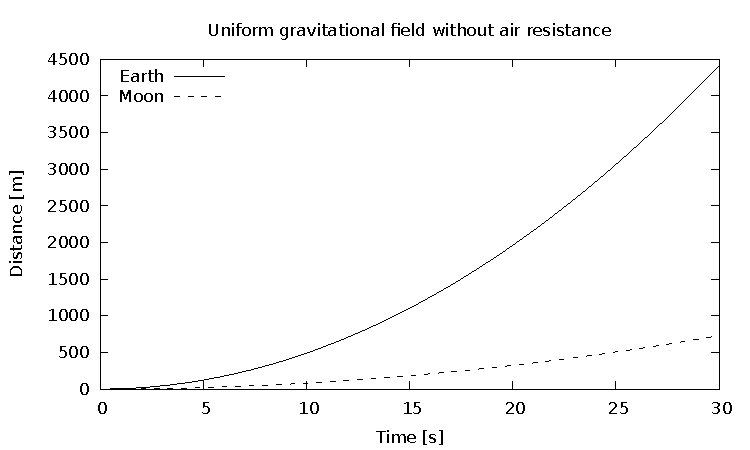
\includegraphics{gnuplot-bw}
% 	\caption{Černobílá varianta obrázku generovaného programem Gnuplot}\label{fig:gnuplot-bw}
% \end{figure}
% 
% \begin{figure}\centering
% 	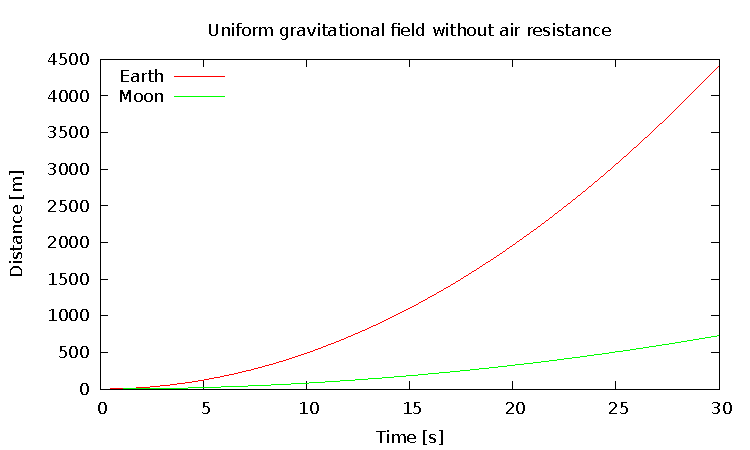
\includegraphics{gnuplot-col}
% 	\caption{Barevná varianta obrázku generovaného programem Gnuplot}\label{fig:gnuplot-col}
% \end{figure}
% 
% 
% \subsection{Tabulky}
% 
% Tabulky lze zadávat různě, např. v~prostředí \verb|tabular|, avšak pro jejich vkládání platí to samé, co pro obrázky -- použijte plovoucí prostředí, v~tomto případě \verb|table|. Například tabulka \ref{tab:matematika} byla vložena tímto způsobem.
% 
% \begin{table}\centering
% 	\caption[Příklad tabulky]{Zadávání matematiky}\label{tab:matematika}
% 	\begin{tabular}{|l|l|c|c|}\hline
% 		Typ		& Prostředí		& \LaTeX{}ovská zkratka	& \TeX{}ovská zkratka	\tabularnewline \hline \hline
% 		Text		& \verb|math|		& \verb|\(...\)|	& \verb|$...$|		\tabularnewline \hline
% 		Displayed	& \verb|displaymath|	& \verb|\[...\]|	& \verb|$$...$$|	\tabularnewline \hline
% 	\end{tabular}
% \end{table}
% 
% % % % % % % % % % % % % % % % % % % % % % % % % % % % 

\chapter{Obsah přiloženého CD}

%upravte podle skutecnosti

\begin{figure}
	\dirtree{%
		.1 readme.txt\DTcomment{stručný popis obsahu CD}.
		.1 exe\DTcomment{adresář se spustitelnou formou implementace}.
		.1 src.
		.2 impl\DTcomment{zdrojové kódy implementace}.
		.2 thesis\DTcomment{zdrojová forma práce ve formátu \LaTeX{}}.
		.1 text\DTcomment{text práce}.
		.2 thesis.pdf\DTcomment{text práce ve formátu PDF}.
		.2 thesis.ps\DTcomment{text práce ve formátu PS}.
	}
\end{figure}

\end{document}
